\documentclass{article}

\usepackage[italian]{babel}
\usepackage[a4paper, margin=2cm]{geometry}
\usepackage{xcolor}
\usepackage{tocloft}
\usepackage{titlesec}
\definecolor{bluscuro}{RGB}{0, 0, 139}  % Definizione di un blu scuro
\usepackage{amsmath}
\usepackage{graphicx}
\usepackage[colorlinks=true, allcolors=bluscuro]{hyperref}
\usepackage{wrapfig}
\usepackage{caption}

\graphicspath{{immagini/}}

% Cambiare il colore delle sezioni
\titleformat{\section}
  {\color{bluscuro}\Large\bfseries} % Stile: colore + grande + grassetto
  {\thesection}{1em}{}

\titleformat{\subsection}
  {\color{bluscuro}\large\bfseries} % Stile: colore + medio + grassetto
  {\thesubsection}{1em}{}

\renewcommand{\cfttoctitlefont}{\color{bluscuro}\huge\bfseries} % Titolo "Indice" in blu e grande

\title{Documentazione Cross}
\author{Martini Matteo 636694}

\begin{document}
\maketitle

\tableofcontents
\newpage

\section{Scelte Progettuali}
Il progetto è stato realizzato seguendo i principi SOLID per garantire modularità, scalabilità e manutenibilità.
\subsection{Organizzazione delle unità di codice}
La suddivisione intensiva in package garantisce la modularità per le varie funzionalità e migliora la fruibilità del codice.
Di seguito verranno elencati i package principali:
\begin{itemize}
    \item \textbf{Client}: contiene le task da eseguire lato Client e la classe che verrà istanziata per usufruire del servizio.
    \item \textbf{Commands}: contiene tutti i comandi che possono essere utilizzati dagli utenti, insieme alla factory per istanziarli.
    \item \textbf{Communication}: contiene i protocolli di comunicazione utilizzati insieme ai tipi di messaggio definiti per la comunicazione.
    \item \textbf{Config}: contiene le classi per configurare Client e Server.
    \item \textbf{Executables}: contiene ServerMain e ClientMain che eseguiranno rispettivamente Server e Client del servizio Cross.
    \item \textbf{JsonAccessedData}: contiene tutti i vari file Json utilizzati per mantenere informazioni persistenti.
    \item \textbf{Server}: contiene le task da eseguire lato Server e la classe che verrà istanziata per creare il Server centrale del servizio Cross.
    \item \textbf{Utils}: contiene varie classi di utilità che semplificano l'esecuzione del codice.
\end{itemize}

\subsection{Comunicazione}
La comunicazione definita nel package \textbf{Communication} contiene i due protocolli utilizzati:

\begin{itemize}
    \item \textbf{TCP}: Protocollo maggiormente utilizzato per la comunicazione Client-Server mediante il quale il Client può inviare richieste al Server. La conessione viene instaurata all'avvio del Client e persiste fino alla chiusura dello stesso o di problemi che causano la chiusura del Server
    \item \textbf{UDP}: Protocollo utilizzato per notificare gli utenti della finalizzazione delle transazioni legate agli ordini da loro piazzati nell'orderbook
\end{itemize}

\subsection{Gestione di Orderbook e Registrazioni}
L'orderbook viene realizzato mediante un file Json diviso in due campi principali \textbf{askMap} e \textbf{bidMap} che contengono i relativi ordini
Questa scelta consente di persistere i dati sugli ordini anche dopo la chiusura del Server, oltre a garantire una relativa semplicita nel caricamento in memoria degli ordini tramite una struttura dati apposita.
\\La gestione delle registrazioni è simile mediante un \textbf{"Userbook"} con una chiave usermap per rendere più agevole la traduzione da Json a struttura dati, inoltre per garantire maggiore sicurezza le password sono state criptate grazie alla libreria \textbf{BCrypt}.

\subsection{Sincronizzazione}
Per garantire consistenza in un ambiente concorrente vengono utilizzati metodi \textbf{synchronized} per proteggere sezioni critiche ed inoltre le varie strutture dati presenti nella collezione \textbf{java.util.concurrent}.

\subsection{Design Pattern}
Il progetto utilizza principalmente la \textbf{Simple Factory} per generare i comandi da inviare al Server.
Questa generazione avviene sul Client sfruttando l'interfaccia \textbf{Values} la quale offre il metodo execute che il Server utilizzerà per eseguire correttamente i vari comandi disponibili. Inoltre questo approccio consente di mantenere invariato il formato di messaggi,\textbf{Message\{Operation,Values\}} che il Client invia al server e facilita l'aggiunta di comandi in quanto è sufficiente creare una nuova implementazione di Values.

\section{Schema Generale dei Thread Attivati}
Il progetto sfrutta il multithreading per gestire la comunicazione Client-Server in maniera efficiente, oltre all'elaborazione asincrona di attività interne
\subsection{Thread Lato Client}
Il client attiva ed usa 3 thread durante il normale funzionamento:
\begin{itemize}
  \item \textbf{SenderThread}: utilizzato per inviare i comandi al server mediante connessione \textbf{TCP}.
  \item \textbf{ReceiverThread}: utilizzato per ricevere le risposte del server mediante connessione \textbf{TCP}.
  \item \textbf{UDPReceiverThread}: utilizzato per ricevere le notifiche legate alle transazioni che riguardano gli ordini piazzati dall'utente mediante connessione \textbf{UDP}.
\end{itemize}
I primi due thread vengono istanziati nella classe ClientClass e persistono le informazioni fino alla chiusura del socket, la scelta di avere due thread separati per invio e ricezione consente di ricevere in maniera asincrona le risposte del server, aiutando quindi a gestire i casi in cui si riscontrano dei problemi sul server richiedendo però l'utilizzo di una variabile per sincronizzare i due thread impedendo così di inviare al massimo 1 messaggio alla volta aspettando così la relativa risposta.
\\ \textbf{UDPReceiverThread} viene istanziato subito dopo la ricezione del primissimo messaggio inviato dal server, che contiene le informazioni su porta e gruppo multicast al quale connettersi per ottenere informazioni sugli ordini.
È stato scelto di utilizzare multicast per semplificare l'implementazione del paradigma Publish-Subscribe per gli ordini; un'altro vantaggio di multicast consiste nel poter assegnare ad ogni ordine dell'orderbook un gruppo multicast, vantaggio che in questo progetto non è stato sfruttato appieno in quanto non richiesto esplicitamente.

\subsection{Thread Lato Server}
Il Server utilizza un \textbf{FixedThreadPool} per gestire i vari client connessi che vengono rappresentati da una \textbf{GenericTask}, inoltre attiva i seguenti Thread:
\begin{itemize}
  \item \textbf{UDPListner}: Thread che si occupa dell'invio delle notifiche secondo il modello Publish-Subscribe.
  \item \textbf{StopOrderChecker}: Thread che si occupa di controllare gli \textbf{StopOrder} piazzati dagli utenti ed eseguirli in caso lo stopprice lo consenta.
  \item \textbf{ClosingTask}: Thread che si occupa di svolgere la chiusura del server in sicurezza quando si riscontrano dei problemi sul server per i quali non si può garantire la fruizione del servizio di trading. 
\end{itemize}
Tutti i thread nominati prima vengono istanziati dalla classe \textbf{ServerClass}, i primi due subito dopo aver fatto la bind dell'indirizzo del socket, mentre l'ultimo viene aggiunto come \textbf{ShutdownHook} alla JVM per consentire di terminare il servizio in maniera sicura in qualsiasi momento si dovesse verificare un problema lato Server per il quale sia richiesta al chiusura, aumentando così al \textbf{Fault Tollerance} del progetto. 
Il timeout viene gestito mediante uno scheduler che dopo 10 minuti esegue un \textbf{DisconnectTask} per disconnettere per inattività il client; questo scheduler viene istanziato da ogni GenericTask per il proprio client.
\newpage

\section{File Java}
Il progetto sfrutta i java package per organizzare meglio i file Java contenenti le classi che verranno usate per fornire il servizio di trading; Di seguito verranno analizzati i vari package ed alcuni file tra i più importanti, motivando le scelte fatte.
\subsection{Communication}
Questo package contiene i protocolli di comunicazione utilizzati dal progetto, insieme ai tipi di messaggio che vengono scambiati tra Client e Server.
I protocolli, come menzionato precedentemente, sono \textbf{UDP} e \textbf{TCP} che vengono realizzati implementando l'interfaccia \textbf{Protocol} che richiede un metodo rispettivamente per invio e ricezione di messaggi ed uno per la chiusura del protocollo;
Inoltre \textbf{TCP} utilizza i metodi forniti da \textbf{Moshi} per realizzare uno scambio di messaggi in formato Json, sfruttando le varie implementazioni dell'interfaccia \textbf{Values}.

\begin{wrapfigure}{r}{0.5\textwidth} % "r" = destra, "l" = sinistra
  \centering
  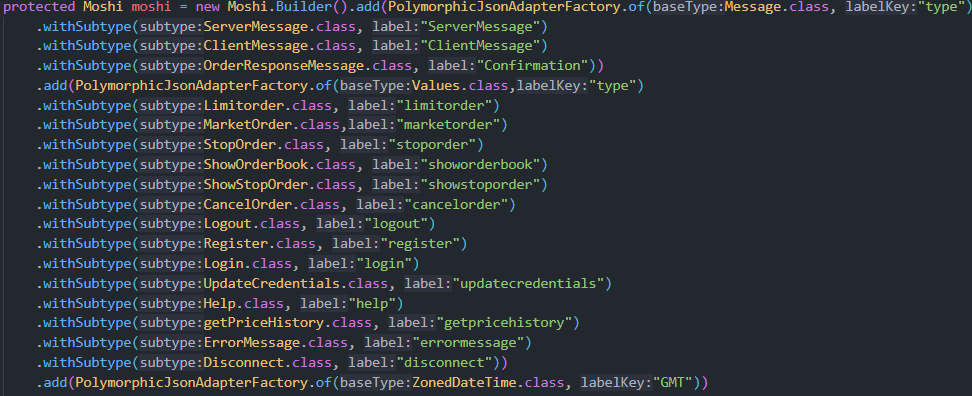
\includegraphics[width=\linewidth]{Moshi-Classi.png} % Assicurati che il nome sia corretto
  \caption{\footnotesize Aggiunta delle sottoclassi di Values}
\end{wrapfigure}

Moshi si è rivelato più facilmente manutenibile rispetto a Gson in quanto non perde le informazioni della sottoclasse di \textbf{Values} incapsulata nel messggio inviato/ricevuto.
\\Questo si è rivelato fondamentale in quanto ha permesso di mantenere la struttura dei messaggi richiesta dalla consegna. Questo si ottiene registrando tutti le Classi o sottoclassi che potrebbero essere passata nei Messaggi ad un builder di moshi tramite \textbf{JsonAdapterFactory}, come si può notare nella figura affianco.
Inoltre per finire la configurazione di Moshi è bastato creare un \textbf{JsonAdapter$<$Message$>$} che, similmente a Gson, si occuperà di serializzare/deserializzare il messaggio in formato Json.

\subsection{Commands}
Questo package contiene tutti i comandi che il Client può inviare al Server e la factory che si occupa di crearli. La creazione avviene lato Client per rispettare il formato dei messaggi da scambiare ed inoltre consente di alleggerire il dei gestori lato Server che si limiteranno ad usare il metodo execute fornito dall'interfaccia \textbf{Values}.
I comandi sono divisi in base al tipo di dato Json che richiedono per essere eseguiti:
\begin{itemize}
  \item \textbf{Credentials}: comandi che aggiungono o modificano informazioni nell'\textbf{Userbook}
  \item \textbf{Order}: comandi che aggiungono o modificano informazioni nell'\textbf{Orderbook}
  \item \textbf{Internal}: comandi che non richiedono alcun tipo di Json e sono utilizzati per operazioni interne, ad esempio i messaggi d'errore.
\end{itemize}
Le strutture dati che rappresentano i file Json verranno poi successivamente aggiunte al comando nel \textbf{GenericTask}, lato Server, prima di essere eseguito.\\
L'unica eccezione è \textbf{getPriceHistory} che richiede lo storico degli ordini per il suo funzionamento però tale file è richeisto nella configurazione del Server in quanto viene usato come risorsa a sola lettura. 
\\Questa scelta di utilizzare sottoclassi di Values e una \textbf{SimpleFactory} semplifica l'aggiunta di nuovi comandi in quanto è sufficiente:
\begin{enumerate}
  \item \textbf{Creare} un classe Java che implementi Values
  \item \textbf{Aggiungere} alla factory la creazione della nuova classe
  \item \textbf{Aggiungere} nel builder di moshi la sottoclasse appena creata
\end{enumerate}

\subsection{Utils}
Questo package contiene le varie classi utilizzate per semplificare la manipolazione dei file Json, le eccezzioni create per gestire i parametri errati nella creazione dei comandi mediante factory ed una cache per il mantenimento in memoria degli ordini evasi durante l'esecuzione di un ordine.
\newpage
\subsection{JsonAccessedData}
Questo package contiene le classi che rappresentano in memoria i file Json, ed i file Json veri e propri ad eccezzione dello storico ordini come discusso precedentemente.

\subsubsection{Orderbook}
L'orderbook è il cuore del servizio offerto in quanto contiene i limitorder piazzati dagli utenti e deve essere sempre acceduto per ogni ordine. È suddiviso in \textbf{askMap} e \textbf{bidMap} dove verranno memorizzati i relativi ordini, mentre gli StopOrder verranno memorizzati in una \textbf{ConcurrentLinkedQueue}.
\subsubsection{Userbook}
L'userbook contiene le informazioni sugli account degli utenti e viene acceduto per poter iniziare ad usare il servizio di trading. È costituito da una \textbf{userMap} che contiene tutti gli utenti, questo è stato fatto per facilitare lettura e scrittura in memoria tramite \textbf{Moshi}. 
\subsubsection{Storico Ordini}
Lo storico ordini sebbene venga trattato come risorsa a sola lettura presenta una struttura singolare che andremo ad analizzare.
\\Viene caricato in memoria come \textbf{TreeMap$<$Integer,TreeMap$<$DayTime,Trade$>$$>$}, dove la chiave Integer della prima TreeMap rappresenta l'anno in cui è avvenuta la transazione, mentre la TreeMap interna ha come chiave la classe \textbf{Daytime} che contiene informazioni su ora giorno e mese in cui è avvenuta la transazione, mentre il valore è rappresentato dal \textbf{Trade} ossia la transazione effettiva.
\textbf{DailyTradeStats} è la classe che viene usata per rappresentare i seguenti parametri registrati giorno per giorno:
\begin{itemize}
  \item Prezzo di apertura
  \item Prezzo di chiusura
  \item Minimo prezzo di una transazione di tipo Ask
  \item Minimo prezzo di una transazione di tipo Bid
  \item Massimo prezzo di una transazione di tipo Ask
  \item Massimo prezzo di una transazione di tipo Bid
\end{itemize}
Questo per consentire una più agevole esecuzione del comando \textbf{getPriceHistory}.

\subsection{Client}
La classe ClientClass, contenuta nel package Client, si occupa di comunicare col server sfruttando il \textbf{multithreading} per poter riceve richieste TCP \textbf{asincrone} dal Server, oltre a predisporre un Thread di ricezione UDP per essere notificato sullo stato delle transazioni. 
Questa è la classe che viene istanziata dal ClientMain per realizzare il client del servizio offerto.

\subsection{Server}
La classe ServerClass, contenuta nel package Server, si occupa di creare il ServerSocket sul quale accetterà le connessioni dei client e che verranno gestite mediante \textbf{GenericTask} che verrà passata al threadpool.\\
GenericTask si occupa quindi di comunicare direttamente col Client e di eseguire i comandi da lui richiesti.

\newpage

\section{Sincronizzazione}
Sfruttando il multithreading è necessario controllare che le sezioni critiche non vengano compromesse da accessi simultanei da parte di più thread,
per fare questo sono state utilizate \textbf{primitive di sincronizzazione} e strutture dati \textbf{Thread-Safe} che verranno elencate e descritte di seguito.
\subsection{synchronized}
La keyword synchronized viene utilizzata per proteggere sezioni di codice critiche, consentendo l'accesso a solo un thread per volta.

\subsection{volatile}
La keyword volatile garantisce la visibilità immediata delle modifiche a variabili condivise tra thread.

\begin{table}[h]
  \captionsetup{justification=raggedright, singlelinecheck=false}
  \caption*{\textbf{Variabili volatile del progetto}}
  \center
  \begin{tabular}{|p{4cm}|p{2cm}|p{7.4cm}|}
    \hline
    \textbf{Variabile} & \textbf{Classe} & \textbf{Utilizzo} \\
    \hline
    \centering canSend   & ClientClass   & Impedire l'invio di più richieste senza prima aver ricevuto una risposta\\
    \hline
    \centering onlineUser   & ClientClass   & Memorizzare il nome utente con cui l'utente si è loggato per personalizzare il prompt\\
    \hline
    \centering cmdSent   & ClientClass   & Memorizzare l'ultimo comando mandato dall'utente al server \\
    \hline
    \centering sigintTermination & ClientClass & Controllare se la terminazione sta avvenendo a causa di un sigInt sul client\\
    \hline
    \centering registerdUsers & ServerClass & Accedere all'userbook\\
    \hline
    \centering orderbook & ServerClass & Accedere all'orderbook\\
    \hline
    \centering progressiveOrderNumber & ServerClass & generare l'orderId degli ordini\\
    \hline
  \end{tabular}
\end{table}

\subsection{ConcurrentHashMap}
La ConcurrentHashMap è una struttura dati ottimizzata per l'accesso concorrente, segmentando la mappa in più 
sezioni per ridurre il blocco globale. È la rappresentazione in memoria dell'Userbook ed è stata scelta in quanto 
non deve essere ordinata e garantisce l'unicità delle chiavi usate, tali chiavi sono rappresentate dall'username scelto dall'utente.

\subsection{ConcurrentSkipListMap}
La ConcurrentSkipListMap è una struttura dati che fornisce una versione Thread-Safe della Skip List, ossia 
una struttura dati probabilistica che permette ricerche con complessità O$($log n$)$ al caso medio 
e mantiene l'ordinamento naturale delle chiavi, se sono implementazioni di comparable, oppure mediante un comparator fornito al costruttore.
Questa struttura è stata utilizzata per rappresentare in memoria \textbf{askMap} e \textbf{bidMap} in quanto devono essere ordinati rispettando:
\begin{enumerate}
  \item \textbf{Prezzo}
  \item \textbf{Timestamp}
\end{enumerate} 
L'ordinamento è mantenuto mediante la classe \textbf{OrderSorting} che implementa \textbf{Comparable} ed inoltre 
\\gli ordinamenti crescente e decrescente vengono implementati mediante un comparator che sfrutta il metodo compareTo implementato dalla classe OrderSorting.

\subsection{ConcurrentLinkedQueue}
La ConcurrentLinkedQueue è una struttura dati non bloccante che rispetta l'ordinamento \textbf{FIFO}, necessario per garantire la corretta priorità agli ordini, progettata per operazioni concorrenti ad alte prestazioni viene utilizzata per matenere gli stoporder in attesa di elaborazione. 
\\La natura lock-free di questa struttura garantisce un elevato throughput anche con un elevato numero di accessi.

\newpage

\section{Utilizzare il Progetto}
Questo capitolo agisce da manuale per l'esecuzione del progetto, per la struttura si rimanda al paragrafo 1.1 .
\subsection{Requisiti di Sistema}

\begin{itemize}
  \item \textbf{Java Development Kit (JDK)}: Versione 8 o superiore.
\end{itemize}

\subsection{Dipendenze Esterne}
  \begin{itemize}
    \item \textbf{Moshi}: Libreria per manipolare oggetti Json.
    \item \textbf{Moshi Adapters}: Libreria aggiuntiva per Moshi che semplifica la gestione di polimorfismi e situazioni complesse nella serializzazione Json.
    \item \textbf{Okio}: Libreria I/O moderna che semplifica ed ottimizza operazioni di input/output, è una dipendenza di Moshi.
    \item \textbf{BCrypt}: Libreria che fornisce la utility per hashing sicuro delle password, indipendenti dal framework Spring Security, oltre alla cifratura e decifratura di chiavi.
    \item \textbf{Apache Commons Lang3}: Libreria che fornisce utility che estendono l'API di Java e che risolvono problemi comuni come gestione di null e manipolazione di stringhe.
    \item \textbf{Apache Commons Logging}: Dipendenza di Apache Commons Lang3.
  \end{itemize}

\subsection{Esecuzione del Progetto}
Il progetto include due componenti principali, ovvero \textbf{Client} e \textbf{Server}, che devono essere avviati separatamente.

\subsubsection{Avvio del Server}
Eseguire il comando: \textbf{java -jar server.jar}
come prima cosa verrà caricato il file \textbf{ServerConfig.json} contenente 
le informazioni necessarie al caricamento dei file Json in memoria, ed indirizzi e porte necessari per instaurare 
le connessioni TCP ed UDP.

\subsubsection{Avvio del Client}
Eseguire il comando: \textbf{java -jar client.jar}
come prima cosa verrà caricato il file \textbf{ClientConfig.json} contenente indirizzi e porta TCP per connettersi al Server.

\end{document}